\newcommand{\source}[1]{\caption*{Source: {#1}} }

\section{Verwandte Arbeiten}\raggedbottom

\subsection{Semantische Segmentierung im medizinischem Bereich}
Bereits in den 90er Jahren wurde sich mit mit Segmentierungsarchitekturen auseinandergesetzt und baselines geschaffen. Zu dieser Zeit leiferten Methoden mim Bereich 'Pattern recogniction' die besten Ergebnisse ( MRI SEGMENTATION: ETHODS AND APPLICATIONS 1995). Die Autoren legten viel Wert auf preprocessing der Daten und nutzen Methoden wie viele, zu der Zeit, State of the Art Modelle (kNN, Maximimun likelihood, 2D feature maps usw.) ausprobiert worden sind (Noise Suppression and Contrast Enhancement, Combination analysis, adaptive filtering usw.). Trotz den Bemühungen wiesen die Modelle nur eine Accuracy von 3\% bis 34\% auf. 

Die Autoren sind davon überzeugt, dass segmentierung eine wichtige Rolle im Beriech der Verarbeitung von MRT Daten darstellen wird und mit wachsender Akzeptanz auf klinischer Seite sowie dem technischen Fortschritt der Hochleistungsrechner es in Zukunft möglich sein wird, akkurate Segmentierungen von MRT Scans im live Betrieb vorzunehmen. 

\subsection{Deep Learning-Techniken für die Segmentierung medizinischer Bilder:
Errungenschaften und Herausforderungen}

Dank der immensen Verbesserung der Rechenleistung der Hardwarecomponenten wurde das Thema Deep Learning immer interessanter und gehört heutzutage zur standard Herangehensweise. Architekturen wie das U-Net Modell haben sich hierbei besonders bewiesen und wurden mit den Jahren nach der Verföffentlichung in 2015 stetig erweitert, so dass es für viele verschiedene medizinische Bereiche Architekturen vorliegen, die auf die jeweiligen Problemstellungen angepasst wurden aber jedoch trotzdem Anwendung auf ähnlichen Gebieten finden können. 

\subsection{Intelligentes Zuschneiden des Inputs}

Dimitrios G. Zaridis et al. fanden heraus, dass das Vorhandensein eines Klassenungleichgewichts, wo der Anteil der Hintergrundpixel dem Anteil des zu segmentierenden Organs überwiegt zu Problemem führen kann. Mithilfe eines Deep Learning Modells haben die Autoren es geschafft, dieses Klassenungleichgewicht zu reduzieren, in dem das Neuronale Netzwerk die gesuchten Organe lokalisiert, das Originalbild zuschneidet und am Ende das Verhältnis von Vorder- und Hintergrundpixeln normalisiert. Dies führte bei allen gängigen Deep Learning Netzwerken zu erheblichen Verbesserung im Bezug des Dice-Scores. U-Net+ und ResU-Net++ wiesen mithilfe dieser Technologie Verbesserungen von bis zu 8\% auf. (A new smart-cropping pipeline for prostate segmentation using deep learning networks)

\section{Grundlagen}\raggedbottom

\subsection{Magen-Darmtrakt}
?? 

\subsection{CNN}
?? 

\subsection{U-Net}
% CNN, Convolution, Maxpooling oder ReLu erklären? 

U-Net wurde im Jahr 2015 von Olag Ronneberger et al. vorgestellt als Segmentierungsarchitektur für den biomedizinischem Bereich und bildet die Baseline dieser Arbeit. Neu in der Herangehensweise ist der Encoder - Decoder Part, die dem Netzwerk ermöglicht räumliche Merkmale anzutrainieren. 
Klassisch handelt es sich um ein Convolutional Neural Network bestehend es aus 5 bis 6 'downsampling' (auch Encoder genannt) Schichten und der gleichen Menge an "upsampling" (auch Decoder genannt) Schichten. 

Eine 'downsample' Operation besteht zum einen aus einer 'Convolution operation'  sowie einer 'Max pooling operation' an deren Ende jeweils eine ReLu Aktivierungsfunktion zum Einsatz kommt. In diesem Schritt lernt das Modell Eigenschaften auf Pixelebene, wie zum Beispiel Formen, Ecken, Kanten. Hierbei halbieren sich die Eingabedimensionen und die Tiefe des Bildes wird erhöht. Das Modell lernt in diesem Schritt das 'was' 

Im Decoder wird das Bild wieder auf seine ursprüngliche Größe mittels 'Transpose Convolution operations' gebracht. Hier ersetzt die transponier Operation die Maxpooling Operation (vergleich Grafik). Dieser Part erlaubt dem Modell das lokalisieren der zuvor gelernten Eigenschaften und gibt eine Maske zurück für jede Klasse, in der 0 der Hintergrund ist und 1 die jeweilige Klasse. 

\subsection{Encoder 1}
Eventuell

\subsection{Encoder 2}
Eventuell


\section{Methodik}\raggedbottom

\subsection{Datenanalyse}
Der Datensatz besteht aus 115 488 Zeilen und enthält drei features: ID, Klasse und einem Run-lenght codierten String, der die Maske enthält. \autoref{tabelle_daten}. Jeder ID sind drei Zeilen gewidmet, jeweils für die drei Klassen. Zu jeder ID existiert ein Graustufen Bild, welche sich im train Ordner befinden: 

input\textbackslash uw-madison-gi-tract-image-segmentation\textbackslash train\textbackslash case101\textbackslash \\case101\textunderscore 
day20\textbackslash scans\textbackslash slice\textunderscore 0001\textunderscore 266\textunderscore 266\textunderscore 1.50\textunderscore 1.50.png

Jedes slice enthält vier Zahlen (z.B. 266\textunderscore 266\textunderscore 1.50\textunderscore 1.50.png), die ersten beiden stehen für die Auflösung des Bildes und die letzten beiden für den physischen Abstand der Pixel. Der Großteil der Aufnahmen stammt von Tag null oder tag eins \autoref{Fig:slice_per_day} und die durchschnittliche Anzahl an Bildern pro Fall beträgt X.

Beim betrachten der Verteilung der Segmentierungen fällt auf, dass das Vorkommen für jede Klasse stark variiert. \autoref{Fig:klassenverteilung}.

\begin{table}[]
	\begin{center}
		\begin{tabular}{lllll}
			\hline
			Index  & ID & Class & Segmentation \\
			\hline \hline
			1     & case134\textunderscore day0\textunderscore slice\textunderscore 0085 	& large\textunderscore bowel 	&  NaN  \\
			2     & case134\textunderscore day0\textunderscore slice\textunderscore 0085 	& small\textunderscore bowel 	&  41591 5 41599 7 41949 27 ...  \\
			3     & case134\textunderscore day0\textunderscore slice\textunderscore 0085 	& stomach 	&  NaN \\
			4     & case123\textunderscore day0\textunderscore slice\textunderscore 0001 	& large\textunderscore bowel 	&  35223 6 74352 7 32312 12 ...   \\
			5     & case123\textunderscore day0\textunderscore slice\textunderscore 0001 	& small\textunderscore bowel 	&  63432 5 12354 7 41949 12 ...  \\
			6     & case123\textunderscore day0\textunderscore slice\textunderscore 0001 	& stomach 	&  NaN \\
			\hline
		\end{tabular}
		\caption{Beispieldaten für zwe slices}\label{tabelle_daten}
	\end{center}
\end{table}

\begin{figure}[!htb]
   \begin{minipage}{0.48\textwidth}
     \centering
     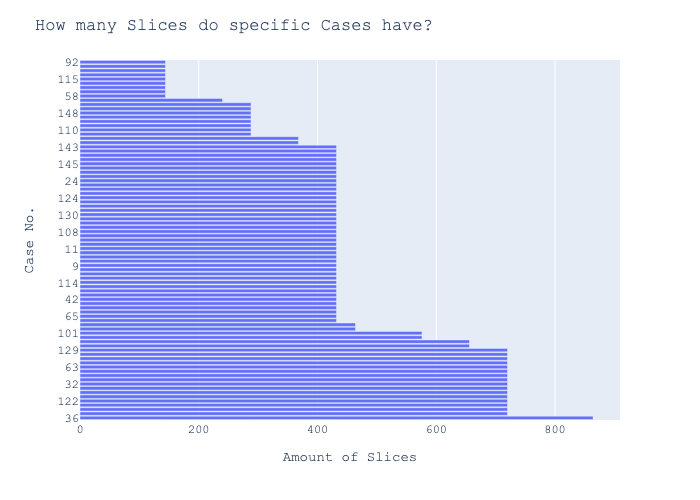
\includegraphics[width=1.2\linewidth]{bilder/slice_per_case}
     \caption{Anzahl Bilder pro Fall}\label{Fig:slice_per_case}
   \end{minipage}\hfill
   \begin{minipage}{0.48\textwidth}
     \centering
     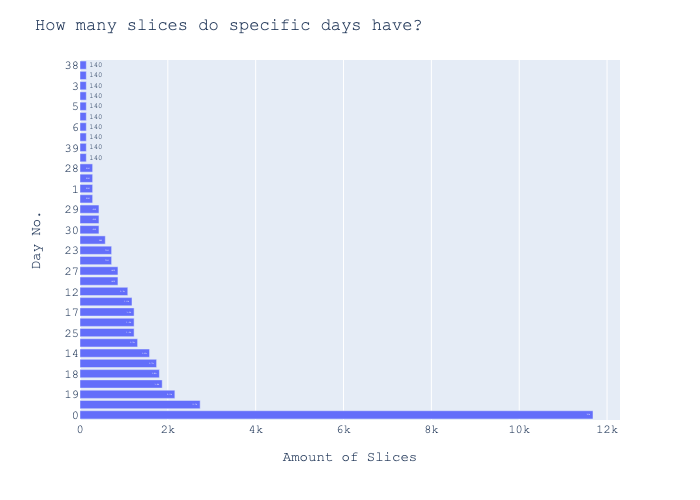
\includegraphics[width=1.2\linewidth]{bilder/slices_per_day}
     \caption{Anzahl Bilder pro Tag}\label{Fig:slice_per_day}
   \end{minipage}
\end{figure}

\subsection{Metadatenextraktion}

Anhand der ID eines jedes Slices war es möglich verschiedene Metadaten dem originalem Dataframe zu entziehen, zudem wurde die gesamtlänge gedrittelt, dadurch dass die Klassen einer ID  zugewiesen worden sind: 
% & rs & re & cs & ce & count & path00 & path01 & path02 & image\textunderscore paths 

\begin{table}[]
 \begin{center}
  \scalebox{0.7}{
   \begin{tabular}{|l|l|l|l|l|l|l|l|l|l|l|l|l|l|}
     \hline
     Idx  & ID &  large\textunderscore bowel & small\textunderscore bowel & stomach & case & day & slice & path & width & height & pixel\textunderscore x & pixel\textunderscore y \\
     \hline \hline
     1     & case134\textunderscore day0\textunderscore slice\textunderscore 0085 	& NaN & 41591 5  ...    & NaN & 134 & 0 & 85 & input\textbackslash  & 266 & 266 & 1.5 & 1.5  \\
     2     & case134\textunderscore day0\textunderscore slice\textunderscore 0086 	& 41591 27 ... & NaN    & NaN & 134 & 0 & 86 & input\textbackslash  & 266 & 266 & 1.5 & 1.5  \\
     3     & case134\textunderscore day0\textunderscore slice\textunderscore 0086 	& NaN & NaN   & NaN & 134 & 0 & 87 & input\textbackslash  & 266 & 266 & 1.5 & 1.5  \\
     \hline
   \end{tabular}
   }
   \caption{Metadaten für drei slices}\label{tabelle_meta_daten}
 \end{center}
\end{table}



\subsection{Algorithmik}
?

\subsection{2.5 dimensionale Daten}
?

\subsection{Intelligentes Zuschneiden}
?

\subsection{Nachbearbeitung }
?

\subsection{Experimente}
Experimente.

\section{Evaluation}\raggedbottom

\section{Fazit}\raggedbottom

\subsection{Ausblick}
Ideen, die es nicht in die Arbeit geschafft haben oder nicht schafffen konnten.


\ifthenelse{\boolean{\biber}}{ % Beispiel um mit Biber zu zitieren (\citet und \citep)
	\citet{Con97} hat ein Buch geschrieben. Es gibt auch andere Arbeiten \citep{PeHe97} die referenziert sind. In Abbildung \ref{fig_Gallien} ist ein Sachverhalt dargestellt.


	1 Autor: \citet{Con97} \hspace*{1cm} \citep{Con97}\\
	2 Autoren: \citet{IWNLP} \hspace*{1cm} \citep{IWNLP}\\
	3 Autoren: \citet{liebeck-esau-conrad:2016:ArgMining2016} \hspace*{1cm} \citep{liebeck-esau-conrad:2016:ArgMining2016}

	Online resource: \citet{ILSVRC2016}
}{ %  Beispiel um klassisch zu zitieren (\cite)
	\cite{Con97} hat ein Buch geschrieben. Es gibt auch andere Arbeiten \cite{PeHe97} die referenziert sind. In Abbildung \ref{fig_Gallien} ist ein Sachverhalt dargestellt.


	1 Autor: \cite{Con97} \hspace*{1cm} \cite{Con97}\\
	2 Autoren: \cite{IWNLP} \hspace*{1cm} \cite{IWNLP}\\
	3 Autoren: \cite{liebeck-esau-conrad:2016:ArgMining2016} \hspace*{1cm} \cite{liebeck-esau-conrad:2016:ArgMining2016}

	Online resource: \cite{ILSVRC2016}
}

\ifthenelse{\equal{\sprache}{deutsch}}{
	\textbf{quotes}:\\
	Ein Beispiel für deutsche Anführungszeichen \glqq quote\grqq.
}{}

\begin{figure}[htb]
	\begin{center}
		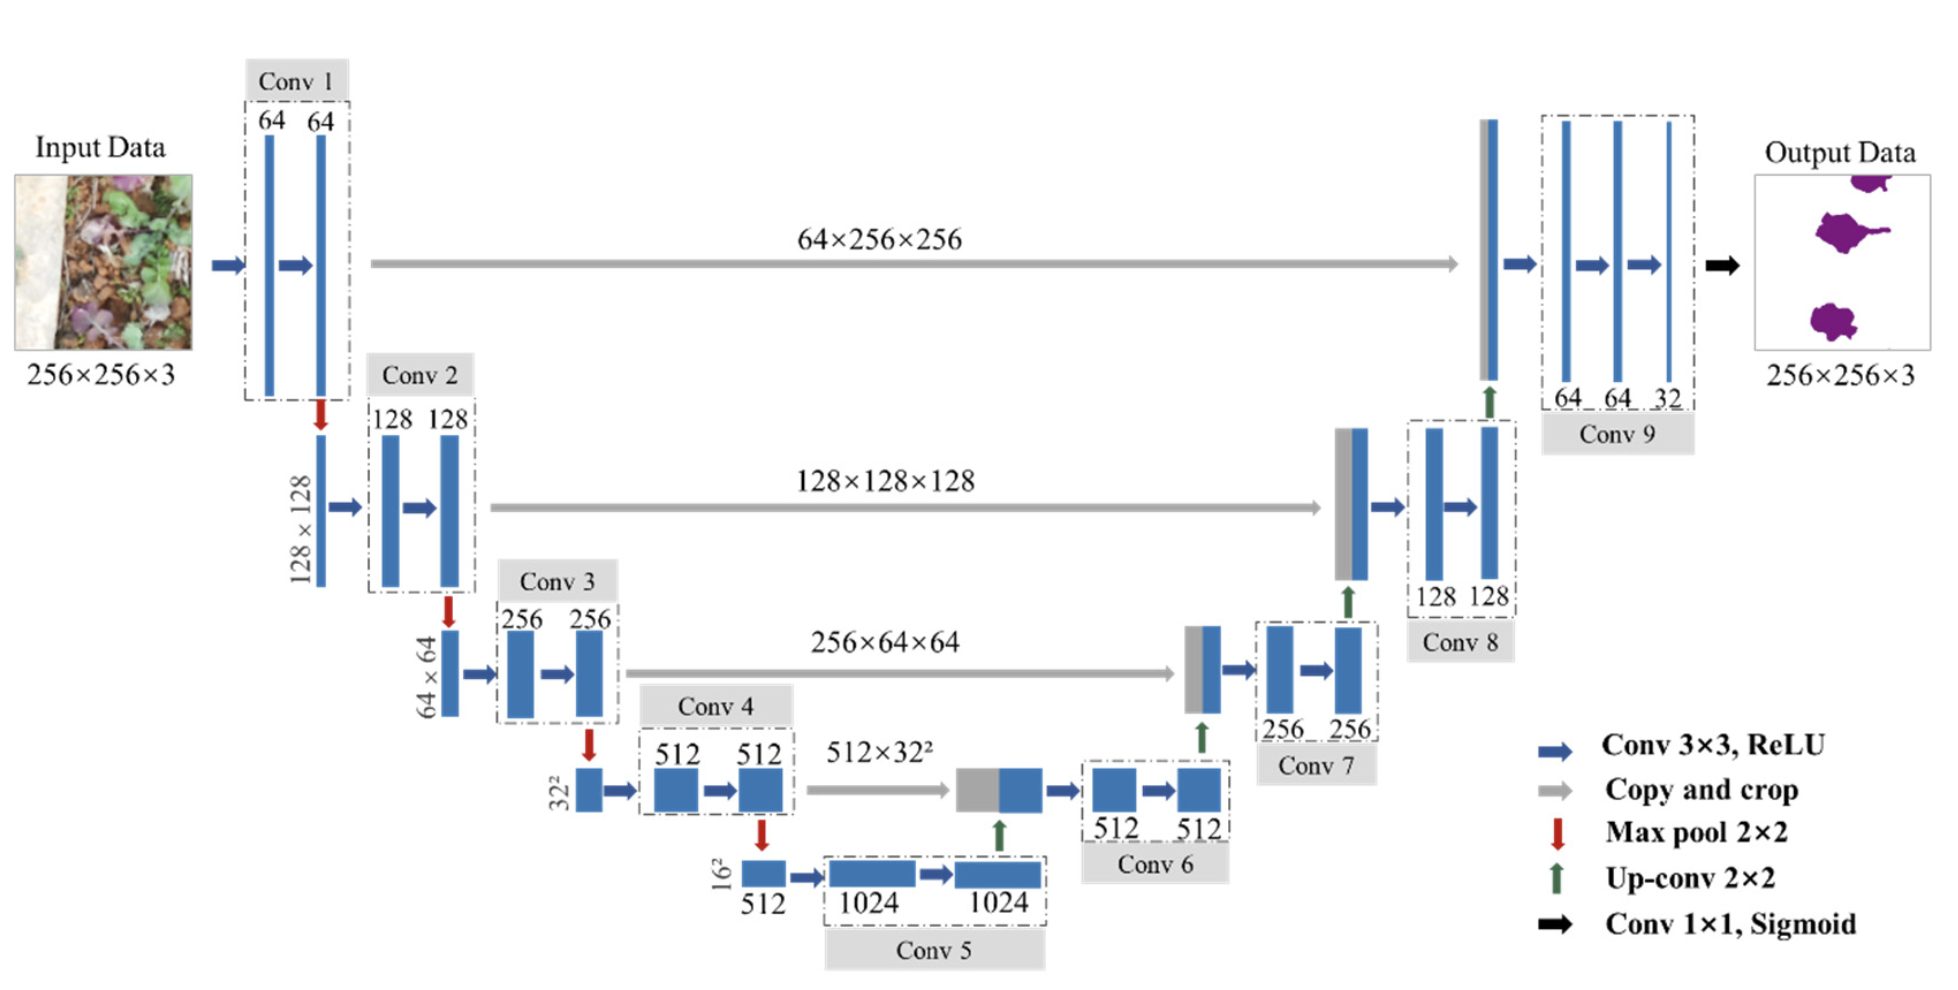
\includegraphics[width=300pt, angle=270]{bilder/u-net-architecture}
		\caption{U-Net Architektur}\label{Fig:unet-diagram}
	\end{center}
\end{figure}

\begin{figure}[htb]
	\begin{center}
		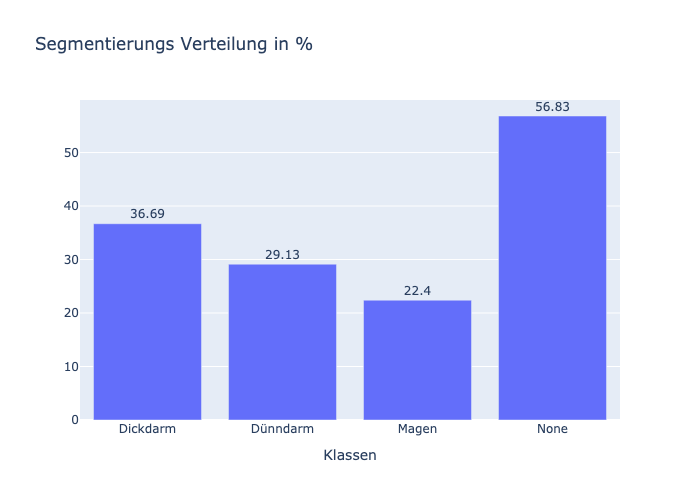
\includegraphics[width=220pt , angle=270]{bilder/segmentation_distribution}
		\caption{Verteilung der Klassen im Testset}\label{Fig:klassenverteilung}
	\end{center}
\end{figure}

\begin{figure}[htb]
	\begin{center}
		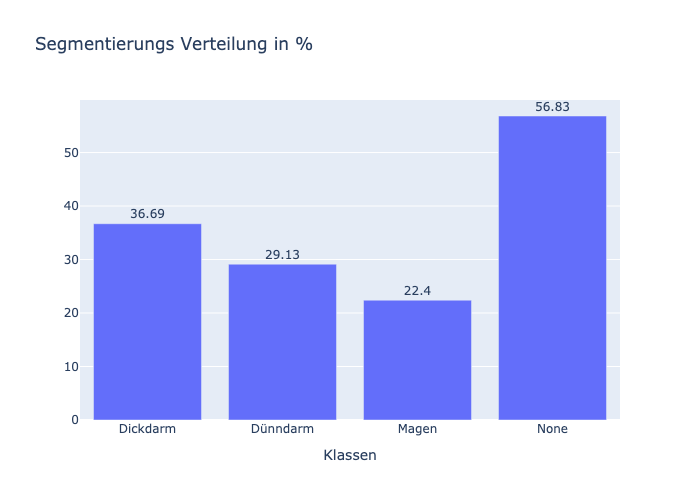
\includegraphics[width=220pt , angle=270]{bilder/segmentation_distribution}
		\caption{Verteilung der Klassen im Testset}\label{Fig:klassenverteilung}
	\end{center}
\end{figure}

\pagebreak